\documentclass[12pt]{article}
\usepackage{geometry}                   
\usepackage{graphicx}
\usepackage{longtable}
\usepackage[latin1]{inputenc}
\usepackage{charter}
\usepackage{amssymb}
\usepackage[american]{babel}
\usepackage{epstopdf}
\DeclareGraphicsRule{.tif}{png}{.png}{`convert #1 `dirname #1`/`basename #1 .tif`.png}
\usepackage{natbib}
\bibpunct[]{(}{)}{,}{a}{}{,}
\bibliographystyle{linquiry2}
\usepackage[normalem]{ulem}
\setlength{\bibsep}{0ex}
\def\qroofpadding{0.2em}
\usepackage{stmaryrd}
\newcommand{\evaluation}[2][]{\ensuremath{\llbracket #2\rrbracket^{#1}}}
\usepackage{Sweave}
\usepackage{pgf}
\usepackage{tipa}
\usepackage{linguex}
\usepackage{tabularx}

\begin{document}

\title{Syntactic complexity from a cross-linguistic perspective: Relative clause extraposition in Russian}
\author{Dillon, Fedorenko, Levy}

\section{Introduction}
\label{sec:intro}

	During sentence comprehension, the identification of the syntactic dependencies that hold between words in the sentence is a crucial step in the process of computing the meaning of a sentence. Theories of syntactic comprehension aim to provide an account of how comprehenders are able to recognize syntactic dependencies quickly and efficiently online. One important source of evidence about the underlying mechanisms comes from results that concern how speakers handle the processing of unambiguous, but complex, structures. Accordingly, much work on syntactic complexity has focused on unbounded filler-gap dependencies where the filler precedes the gap, such as that see in English \textit{wh}-movement and relative clauses (SUPER LONG CITATIONS LIST). Research on non-local filler-gap dependencies has been critical to the development of theories of syntactic comprehension, providing insight into the role of working memory (CITATIONS), predictability (CITATIONS), and structural complexity (CITATIONS) in sentence comprehension.  
	
	In more recent work, the study of rightward movement constructions has been brought to bear on theories of online sentence comprehension (CITATIONS) (footnote: we use movement in a pre theoretical sense to refer to any apparent displacement of a constituent from its canonical position in the sentence). Rightward movement constructions share a number of features that make them attractive objects of study from the point of view of online processing. Levy et al (2012) point out that in many cases rightward movement leads to a syntactic dependency that is formally more complex than dependencies created by leftward movement. For instance, take the process of relative clause extraposition, which displaces a relative clause from its host noun by placing it to the right of its `base' position. This configuration leads to a \textit{non-projective} or crossed syntactic dependencies. This is clearly visible in \ref{dep}, which gives a schematic view of the word-to-word dependencies in \ref{rcex} in the style of Dependency Grammar:
	
	   	\ex.	\label{rcex} \textsc{RC extraposition}: The senator attacked a reporter \_  yesterday  who made an error . (TO BE DRAWN)

	 Here the dependency between \textit{attacked} and \textit{yesterday} can be seen to intersect or cross the dependency between \textit{reporter} and \textit{who}. Crossed dependencies arise when the span of a dependency is partially, but not entirely, contained within the span of the other dependencies in the sentence.  Crossed dependencies imply the presence of noncontinuous constituents. The presence of noncontinuous constituents in natural language has long been taken as one argument that the grammars of natural languages are more powerful than the class of context-free grammars (CITATIONS). The greater formal complexity of non-projective grammars means   e.g. the complexity of tabular parsing algorithms is significantly greater for grammars that allow for non-projective dependencies compared to those that do not (see CITATIONS; but note that it is not clear that this difficulty extends to incremental parsing algorithms c.f CITATION). In several studies, the presence of crossed dependencies has been argued to result in greater processing complexity than the processing of nested dependencies (CITATIONS: Bach, Hale).
	 
	From the point of view of online comprehension, rightward movement presents a number of interesting difficulties even in configurations where non-projectivity does not obtain. Most obviously, the surface order of the filler (the right-displaced constituent) and the gap (its base position) are reversed from the filler-gap order seen in English \textit{wh}-movement and relative clause constructions. Additinoally, the gaps in \ref{rightmove} all contain examples of what what Fodor (CITATION) called a \textit{doubtful gap}: gaps whose existence may not be reliably inferred in an incremental parse of the string given the material that precedes the gap. In the absence of reliable cues to the presence of a gap in rightward movement dependencies, there is a question of if and when the parser will actively predict a gapped analysis. If the parser does not actively predict a gap, then a further question arises  of how the parser is able to identify the correct gap position for the displaced constituent.
	
	\ex.	\label{rightmove}
		\a.	\label{hnps} \textsc{heavy NP shift}: The senator attacked \_ yesterday [ the reporter who made an error ]
		\b.	\label{rcex} \textsc{RC extraposition}: The senator attacked a reporter \_  yesterday [ who made an error ]. 
		\c.	\label{ppex} \textsc{PP extraposition}: The senator attacked a reporter \_  yesterday [ from upstate New York's Adirondack region ]. 
		\d.	\label{compex} \textsc{clausal extraposition}: The senator said  \_ yesterday [ that the reporter made made an error ]. 
		\e.	\label{comparex} \textsc{comparative extraposition}: The senator attacked more reporters  \_ yesterday [ than I could even count ]. 

	Studies of rightward movement dependencies have shown that comprehenders incrementally posit a gap only under very limited conditions in examples like \ref{rightmove}. The exact conditions that allow comprehenders to predictively construct a gapped analysis are somewhat unclear. For instance, Staub, Clifton and Frazier (CITATION) investigated the processing of heavy noun phrase shift (HNPS), a syntactic alternation that involves shifting the object of a verb rightward over some intervening constituent. They found that the comprehender's willingness to adopt an HNPS analysis when she encounters a verb with a missing direct object is modulated by the strength of the transitivity bias of that verb. Comprehenders were shown to adopt an HNPS parse only when they encountered a verb that is obligatorily transitive, as in \ref{stauboblig}. For verbs that allowed both transitive and intransitive subcategorization frames (as in \ref{stauboptional}), comprehenders took a missing argument as a cue to an intransitive use of the verb, and did not project a HNPS analysis. This pattern suggests the comprehenders prioritize thematically complete analyses of partial input over those that contain missing arguments. This finding appears to suggest that a strong probabilistic bias for a gap following a verb is not enough to overcome a bias favoring maximal incremental interpretation. Staub and colleagues conclude that comprehenders only predict an HNPS analysis at the gap only when the grammar requires that there be a gap.

		\ex.	\label{hnpsstaub}
		\a.	\label{stauboblig} \textsc{obligatory gap}: Jack praised \_ from the stands [ his daughter's attempt to shoot a basket ].
		\b.	\label{stauboptional} \textsc{optional gap}: Jack watched \_ from the stands [ his daughter's attempt to shoot a basket ]. 

	Levy, Fedorenko, Breen and Gibson (CITATION) investigated the processing of relative clause extraposition in English. Across two self-paced reading experiments, they showed that processing an extraposed relative clause was associated with greater processing difficulty. This pattern of results was observed for extraposition from subject (\ref{levysubj}), as well as extraposition from object (\ref{levyobj}). 
	
			\ex.	\label{levysubj}
					\a.	 \textsc{in situ}: After the show, a performer who really impressed the audience came on and everyone went wild with applause.
					\b.	 \textsc{extraposed}: After the show, a performer \_ came on [ who really impressed the audience ] and everyone went wild with applause.

				\ex.	\label{levyobj}
					\a.	 \textsc{vp attached, adjacent }: The reporter interviewed the star about the movie which was filmed in the jungles of Vietnam.
					\b.	 \label{levyobj:b} \textsc{vp attached, non-adjacent}: The reporter interviewed the star \_ about the movie [ who was filmed in the jungles of Vietnam ] .
					\c.	 \textsc{np attached, adjacent}: The reporter interviewed the star of the movie which was filmed in the jungles of Vietnam.
					\d.	  \label{levyobj:d} \textsc{np attached, non-adjacent}: The reporter interviewed the star of the movie who was filmed in the jungles of Vietnam.
	
	In both subject extraposition and extraposition from object cases, Levy and colleagues observed increased reading times in the relative clause region when it was extraposed compared to when it was in-situ. These results are compatible with those of Staub and colleagues, and they suggest that readers do not generally incrementally posit a gap of rightward movement. Importantly, the comparison in \ref{levyobj} indicates that the difficulty with extraposition reflects more than simple linear distance between a relative clause and the head noun it modifies. That is, in both \ref{levyobj:b} and \ref{levyobj:d} the number of words between the head noun \texit{star} and the the relative pronoun is the same, but only \ref{levyobj:b} is a true instance of RC extraposition. In \ref{levyobj:d}, the NP attachment of the PP \textit{of the movie} means that the relative clause may be parsed in-situ, modifying the constituent \texitit{the star of the movie}. Levy et al found an interaction in reading times at the relative clause region, such that \ref{levyobj:b} was associated with significantly longer reading times. They interpreted this as processing difficulty associated with the recognition of an extraposition dependency.

	Levy and colleagues further asked is comprehenders could utilize syntactic cues to incrementally posit a gap in examples like \ref{levyobj:b}. They manipulated the predictability of a relative clause postmodifier by contrasting NPs introduced by the definite determiner with those introduced by \textit{only those}. Both corpus and offline completion data suggested a strong preference for a relative clause postmodifier for \textit{only those} compared to \textit{the}. They predicted that this preference would lead comprehenders to anticipate a relative clause postmodifier, leading to eased processing of the extraposed relative clause. They tested this prediction with sentences like the following:
	
					\ex.	\label{levyonlythose}
					\a.	\textsc{weak expectation, in situ}: The chairman consulted the executives about the company which was acquired recently by an aggressive rival firm.
					\b.	\textsc{weak expectation, extraposed}: The chairman consulted the executives \_ about the company [ who was acquired recently by an aggressive rival firm ] .
					\c.	\textsc{weak expectation, in situ}: The chairman consulted only those executives about the company which was acquired recently by an aggressive rival firm.
					\d.	\textsc{weak expectation, extraposed}: The chairman consulted only those executives \_ about the company [ who was acquired recently by an aggressive rival firm ] .

	In conditions where the definite lead to a weak expectation for a post-modifier, they again observed a sizable reading time slowdown for extraposed relative clauses compared to their in-situ counterparts. However, when cued with \textit{only those}, there was no difference in reading times between in-situ and extraposed relative clauses. Like the results of Staub et al, this pattern shows that comprehenders can utilize strong predictive cues to infer the presence of a gap before the rightward-moved filler is encountered. The prediction of the dependency leads to faster processing. However, Levy and colleagues argued that comprehenders did not need to be forced to adopt a gapped analysis by their grammar; instead, graded probabilistic cues are sufficient to cause comprehenders to predict a gapped analysis. This finding contrasts with the finding of Staub and colleagues, who found that comprehenders would not entertain an HNPS analysis for an optionally transitive verb no matter how strong its transitivity bias was.	
	
	 Much of the existing experimental evidence that demonstrates processing difficulty for extraposed relative clauses and other rightward movement constructions comes from English (but see CITATIONS for German). Because English is a language that relies overwhelmingly on word order cues to underlying syntactic structure (CITATIONS), one might question the generality of the results reported by Levy and colleagues. In particular, it is possible to view the penalty associated with extraposed structures as reflecting a violation of highly ranked word order cues. If this is correct, then we expect the processing difficulty associated with extraposition to hold only of languages that have relatively strong reliance on word order. 	 
	 
	 %% Paragraph on Russian goes here. Is there corpus data on RC extraposition on Russian?

	 In the present study, we test whether RC extraposition causes processing difficulty in Russian using configurations that are similar to those seen in English. If Russian speakers do not experience difficulty with RC extraposition, then this result would indicate that the difficulty observed with RC extraposition is a reflection of English's heavy reliance on surface word order cues. On the other hand, if Russian patterns like English, then this strengthens the conclusion of Levy and colleagues that difficulty with extraposition reflects the relative unpredictability of extraposed RCs. 
	  
%%% All the primary analysis routines are in mainAnalysis.R




\section{Experiment}
\label{sec:experiment}

\subsection{Participants}
\label{sec:participants}

Seventeen native Russian speakers living in or visiting the United
States participated in this experiment at the University of California
at San Diego for cash compensation.  None had arrived in the United
States before age 13, and all reported that they continue to use
Russian on a regular basis and consider it the language they are most
comfortable with.
% 2.2.1. Materials

\subsection{Materials}
\label{sec:materials}


Twenty items (listed in full in the Appendix) were constructed following XXX
pattern.  Each participant saw only one of the four conditions of each
item according to a Latin square design.  These experimental stimuli
were interleaved with 32 items from an unrelated experiment and 52
random fillers such that no two experimental sentences were seen
consecutively.

\section{Sample Stimulus}
\label{sec:sample-stimulus}


%\selectlanguage{russian}
\ex. 
\ag. ???????? ???????? ??????????? ??????, ??????? ??????? ??????? ?? ?????????.\\
 {Parent.\masc.\nom} called {teacher.\fem.\dat} {class.\masc.\gen}, {which.\masc.\nom} won recently at Olympiad.\\
``The parent called the teacher of the class$_i$ that$_i$ recently won at the Olympiad.''
\bg. ???????? ???????? ??????????? ??????, ??????? ???????? ?????? ??????????? ????????.       \\
 {Parent.\masc.\nom} called {teacher.\fem.\dat} {class.\masc.\gen}, {who.\fem.\nom} lowered grades {foreign.\pl.\dat} {student.\pl.\dat}.\\
``The parent called the teacher$_i$ of the class who$_i$ lowered the foreign students' grades.''
\cg. ???????? ???????? ??????????? ?\_??????, ??????? ??????? ??????? ?? ?????????.\\
 {Parent.\masc.\nom} called {teacher.\fem.\dat} {about\_class.\masc.\prep}, {who.\masc.\nom} won recently at Olympiad.\\
``The parent called the teacher about the class$_i$ that$_i$ recently won at the Olympiad.''
\dg. ???????? ???????? ??????????? ?\_??????, ??????? ???????? ?????? ??????????? ????????. \\
 {Parent.\masc.\nom} called {teacher.\fem.\dat} {about\_class.\masc.\gen}, {who.\fem.\nom} lowered grades {foreign.\pl.\dat} {student.\pl.\dat}.\\
``The parent called the teacher$_i$ of the class who$_i$ lowered the foreign students' grades.''
\z.
%\selectlanguage{english}

%%% What were the comprehension questions like? One after every item? Did they require readers to resolve the RC attachment?


\subsection{Procedure}
\label{sec:procedure}


Sentences were presented to participants in a non-cumulative
word-by-word moving-window self-paced procedure on a PC laptop
computer running the Linger software \citep{rohde:lingermanual}. Each
trial began with a series of dashes displayed on the computer screen
in place of the words in the sentence. The first press of the space
bar revealed the first word in the sentence, and each subsequent press
of the space bar revealed the next word in the sentence and masked the
previous word. Punctuation was displayed together with the word
preceding it.  The times between button presses were recorded to the
nearest millisecond.  Each sentence was followed by a yes-or-no
comprehension question probing the participant's understanding of the
content of the sentence.  Written instructions in Russian were given
at the outset of the experiment.

\subsection{Data Analysis}
\label{sec:analysis}

Experimental sentences were divided into nine regions of interest as indicated in XXX. Raw reading times were analyzed independently within each region. Prior to analysis, RTs greater than 5000 ms or less than 100ms were excluded. After removing extreme outliers, RTs were further trimmed by removing observations that were more than three standard deviations from a condition mean within a given region. Trials that were incorrectly answered were not excluded from further analysis. This led to a rejection of 109 data points (3.6 \% of the data overall). Response time data were analyzed linear mixed effects (LME) models. The fixed effect structure of all LME models consisted of the experimental factors \textsc{structure}, \textsc{locality}, and their interaction, using simple difference coding (\textsc{structure}: -0.5 for VP attachment,  0.5 for NP attachment;  \textsc{locality}: 0.5 for local attachment, -0.5 for non-local attachment). All mixed effects models used participants and items as random effects, with random intercepts and slopes for all fixed effects (following \cite{barr2013}). In case the model with maximal random effects structure failed to converge, slopes for the interaction term were removed. Accuracy data were analyzed using mixed effects logistic regressions with identical fixed and random effect structure. \textit{p}-values were estimated from model \textit{t}-values by approximation to the standard normal distribution (\cite{baayen2008}).   
  
\subsection{Results}
\label{sec:results}

\subsubsection{Comprehension Accuracy}
\label{sec:acc}

Accuracy on comprehension questions was high, indicating that participants attended to the task. By condition accuracies are provided in \ref{acctable}. Logistic mixed effects modeling of the results indicate no significant differences between conditions. 

% latex table generated in R 3.0.2 by xtable 1.7-1 package
% Thu May 22 11:46:14 2014
\begin{table}[ht]
\centering
\begin{tabular}{rll}
  \hline
 & Local & Non-local \\ 
  \hline
NP & 0.94 (0.02) & 0.95 (0.03) \\ 
  VP & 0.96 (0.03) & 0.94 (0.03) \\ 
   \hline
\end{tabular}
\caption{Mean accuracy by condition for Experiment 1. By-participant standard errors in parentheses.} 
\end{table}
\subsubsection{Reading Times}
\label{sec:rts}

% latex table generated in R 3.0.2 by xtable 1.7-1 package
% Thu May 22 11:46:14 2014
\begin{table}[ht]
\centering
{\scriptsize
\begin{tabularx}{\textwidth}{rlllllllll}
  \hline
 & 1 & 2 & 3 & 4 & 5 & 6 & 7 & 8 & 9 \\ 
  \hline
1 & 637.5 (54) & 704.8 (74) & 856 (108) & 864.6 (93) & 718.6 (64) & 756.6 (59) & 583.6 (52) & 669.6 (53) & 975.9 (84) \\ 
  2 & 618.6 (48) & 725.8 (79) & 891.4 (105) & 861.4 (91) & 677.2 (59) & 721.5 (55) & 578.5 (33) & 667.5 (55) & 975.4 (82) \\ 
  3 & 663.4 (68) & 729.6 (73) & 904.3 (117) & 897.6 (80) & 743.7 (56) & 686.7 (58) & 566.3 (38) & 659.8 (51) & 950 (86) \\ 
  4 & 648.5 (62) & 735.1 (89) & 897.8 (112) & 882.1 (84) & 777.8 (77) & 900.2 (88) & 694.6 (58) & 622.9 (42) & 1136.4 (108) \\ 
   \hline
\end{tabularx}
}
\caption{Mean RTs in each region for Experiment 1. By-participant standard errors in parentheses.} 
\end{table}
Mean RTs in each region, along with by-participant standard error, is presented in \ref{rttable} and in \ref{rtfig}. Prior to the critical relative pronoun region, no significant effects of any experimental fixed effects were found. In the region immediately following the relative pronoun (region 6), mixed effects modeling showed a significant effect of \textsc{locality} ($\beta$ = -93 ($\pm$ 55), $p <$ 0.1), and a significant interaction of \textsc{locality} and \textsc{structure} ($\beta$ = 245 ($\pm$ 122), $p <$ 0.05). In region 7, there was a marginal effect of \textsc{locality} ($\beta$ = -62 ($\pm$ 34), $p <$ 0.1), as well as a marginal interaction \textsc{locality} and \textsc{structure} ($\beta$ = 128 ($\pm$ 68), $p <$ 0.1). Additionally, in region 9 there was a significant interaction of \textsc{locality} and \textsc{structure} ($\beta$ = 230 ($\pm$ 126), $p <$ 0.1), as well as a marginal effect of \textsc{locality} ($\beta$ = -116 ($\pm$ 73), $p <$ 0.112051114916849).

The critical interaction at region 6 was resolved by fitting a second LME model that used nested contrasts to estimate the effect of \textsc{locality} within each level of the \textsc{structure} factor. The results of this model indicate a significant effect of locality for VP attachment conditions ($\beta$ = -216 ($\pm$ 99), $p <$ 0.05). There was no significant effect of locality for NP attachment conditions ($\beta$ = 29 ($\pm$ 60), $p =$ 0.629).


\begin{figure}
\begin{center}
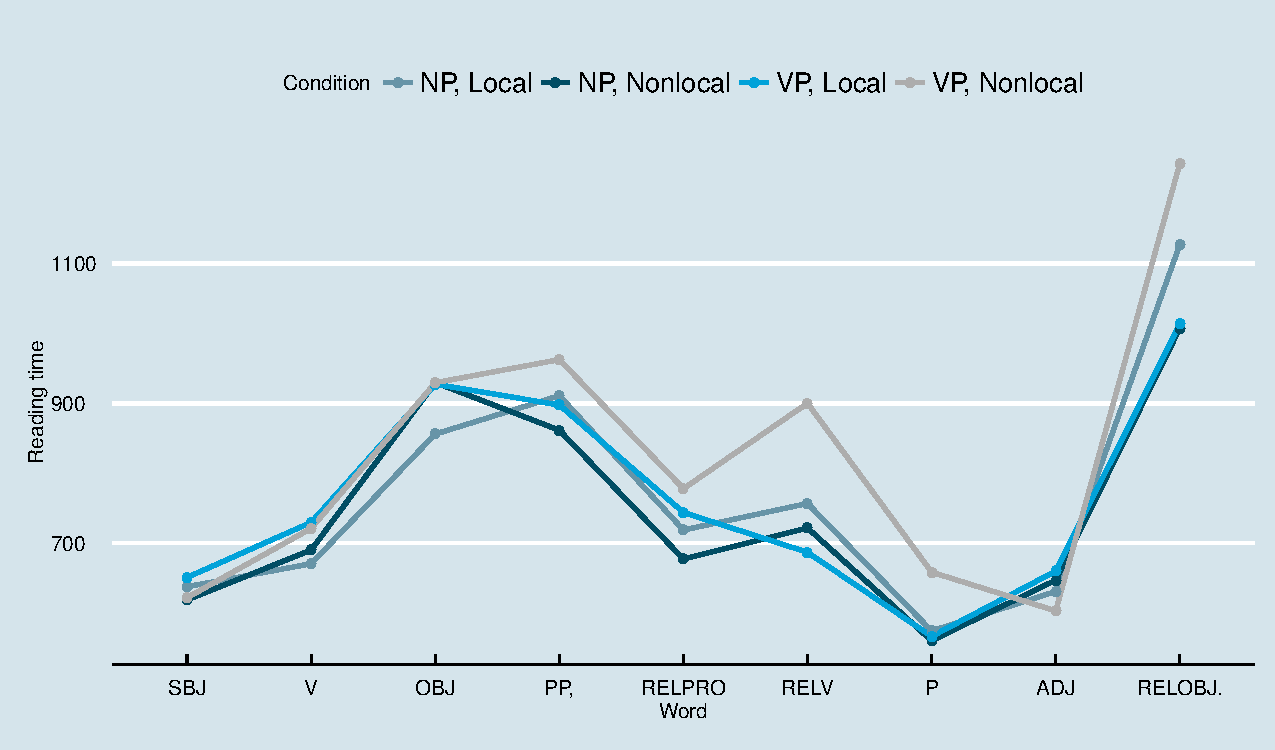
\includegraphics{russian-extraposed-rcs-mainplot}
\end{center}
\caption{Mean reading times in Experiment 1. Error bars represent standard error by participants.}
\label{rtfig}
\end{figure}


\section{Discussion}
\label{sec:experiment}

\subsection{Summary of results}

	%% Compare to size of effect in Levy et al Expt 2

\bibliographystyle{apalike}
\bibliography{russian-extraposed-rcs}

\appendix
\section{Experimental materials}




\end{document}

%%% Local Variables: 
%%% mode: latex
%%% TeX-master: t
%%% End: 
